\documentclass[aspectratio=169,12pt]{beamer}
\usetheme{Madrid}
\usecolortheme{dolphin}
\usefonttheme{professionalfonts}
\setbeamertemplate{navigation symbols}{}
\setbeamertemplate{footline}{}

\usepackage[T1]{fontenc}
\usepackage[utf8]{inputenc}
\usepackage{graphicx}
\usepackage{amsmath,amssymb}
\usepackage{hyperref}
\usepackage{physics}
\usepackage{braket}

\title[]{Quantum Teleportation}
\author{JAMOTTE Maxime, SCHOONEN Cédric}
\institute{Digital Learning Hub}
\date{}

\begin{document}

\begin{frame}
  \titlepage
\end{frame}

\begin{frame}{Reminder: Bell pair, $C_X^{}$ and $C_Z^{}$}
  \begin{columns}[T,onlytextwidth]
    \column{0.6\textwidth}
    \begin{itemize}
      \item Create the Bell pair $\frac{1}{\sqrt 2}(\ket{00} + \ket{11})$.\\~\\
      \item Gate $C_X^{}$: applies $X$ to a qubit if the other is in state $\ket{1}$, otherwise does nothing.\\~\\
      \item Gate $C_Z^{}$: applies $Z$ to a qubit if the other is in state $\ket{1}$, otherwise does nothing.
    \end{itemize}
    \column{0.35\textwidth}
    \centering
    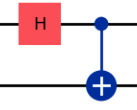
\includegraphics[width=0.6\linewidth]{../figures/bell_pair_crop.png}
  \end{columns}
\end{frame}

\begin{frame}{Teleportation circuit}
  \begin{itemize}
    \item Alice has two qubits: $\ket \psi$ and one of the entangled qubits.
    \item Bob has the other entangled qubit.
    \item The entangled qubits form the Bell pair $\frac{1}{\sqrt 2}(\ket{00} + \ket{11})$.
  \end{itemize}
  \begin{figure}
    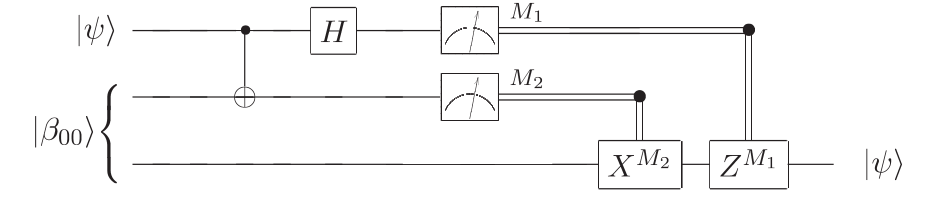
\includegraphics[width=\linewidth]{../figures/teleportation.png}
  \end{figure}
\end{frame}

\begin{frame}{Alternative circuit compatible with a QPU}
    \begin{itemize}
      \item We want to implement this circuit on a QPU.\\~\\
      \item Commands such as \texttt{if} cannot be implemented as on a classical computer (not Python).\\~\\
      \item We therefore need to produce an alternative circuit, where measurements are done at the end of the circuit.
    \end{itemize}
\end{frame}

\begin{frame}{Alternative circuit compatible with a QPU}
    \centering Do a pull (Github)
\end{frame}

\begin{frame}{Exercise: teleportation and run on QPU}
    \begin{itemize}
      \item Teleport the state $\ket \psi = \ket 1$ using the Bell pair $\frac{1}{\sqrt 2}(\ket{00} + \ket{11})$ 
      and gates $C_X$ and $C_Z$.\\~\\
      \item Measure the three qubits at the end of the circuit.\\~\\
      \item Test your circuit with \texttt{Aer} (1000 shots).\\~\\
      \item Present the results in a histogram and interpret the results.\\~\\
      \item After verification, send your circuit to a QPU.
    \end{itemize}
\end{frame}  

\begin{frame}{Circuit that will run on the QPU}
    \begin{figure}
    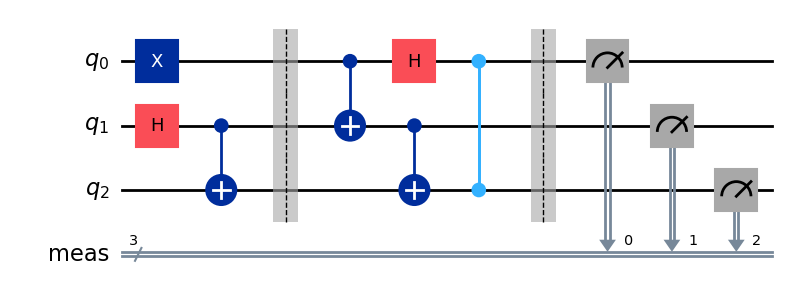
\includegraphics[width=\linewidth]{../figures/teleportation_alternatif.png}
  \end{figure}
\end{frame}  
     

\end{document}
